\documentclass[fleqn,addpoints]{exam}
\usepackage{amsmath}
\usepackage{graphicx}
\usepackage{cancel}
\usepackage{polynom}
\usepackage{float}

\printanswers

\ifprintanswers
\usepackage{2in1, lscape}
\fi

\title{Math 113 Chapters Seven and Ten Exam}
\author{}
\date{August 4, 2010}

% \oddsidemargin 0in
% \topmargin -0.5in
% \textwidth 6.5in

% \extrawidth{-1 in}
% \setlength{\mathindent}{0in}

\begin{document}

\maketitle

\ifprintanswers
\else
\vspace{0.2in}
\makebox[\textwidth]{Name:\enspace\hrulefill}
\vspace{0.2in}

\begin{center}
\gradetable[h][pages]
\end{center}

\fi

\section{Graphing}

For problems \ref{graph:first}-\ref{graph:last}, graph each equation.

\begin{questions}

% \question[5] \( y = \dfrac{1}{2} x + 3\)

% \begin{figure}[H]
%   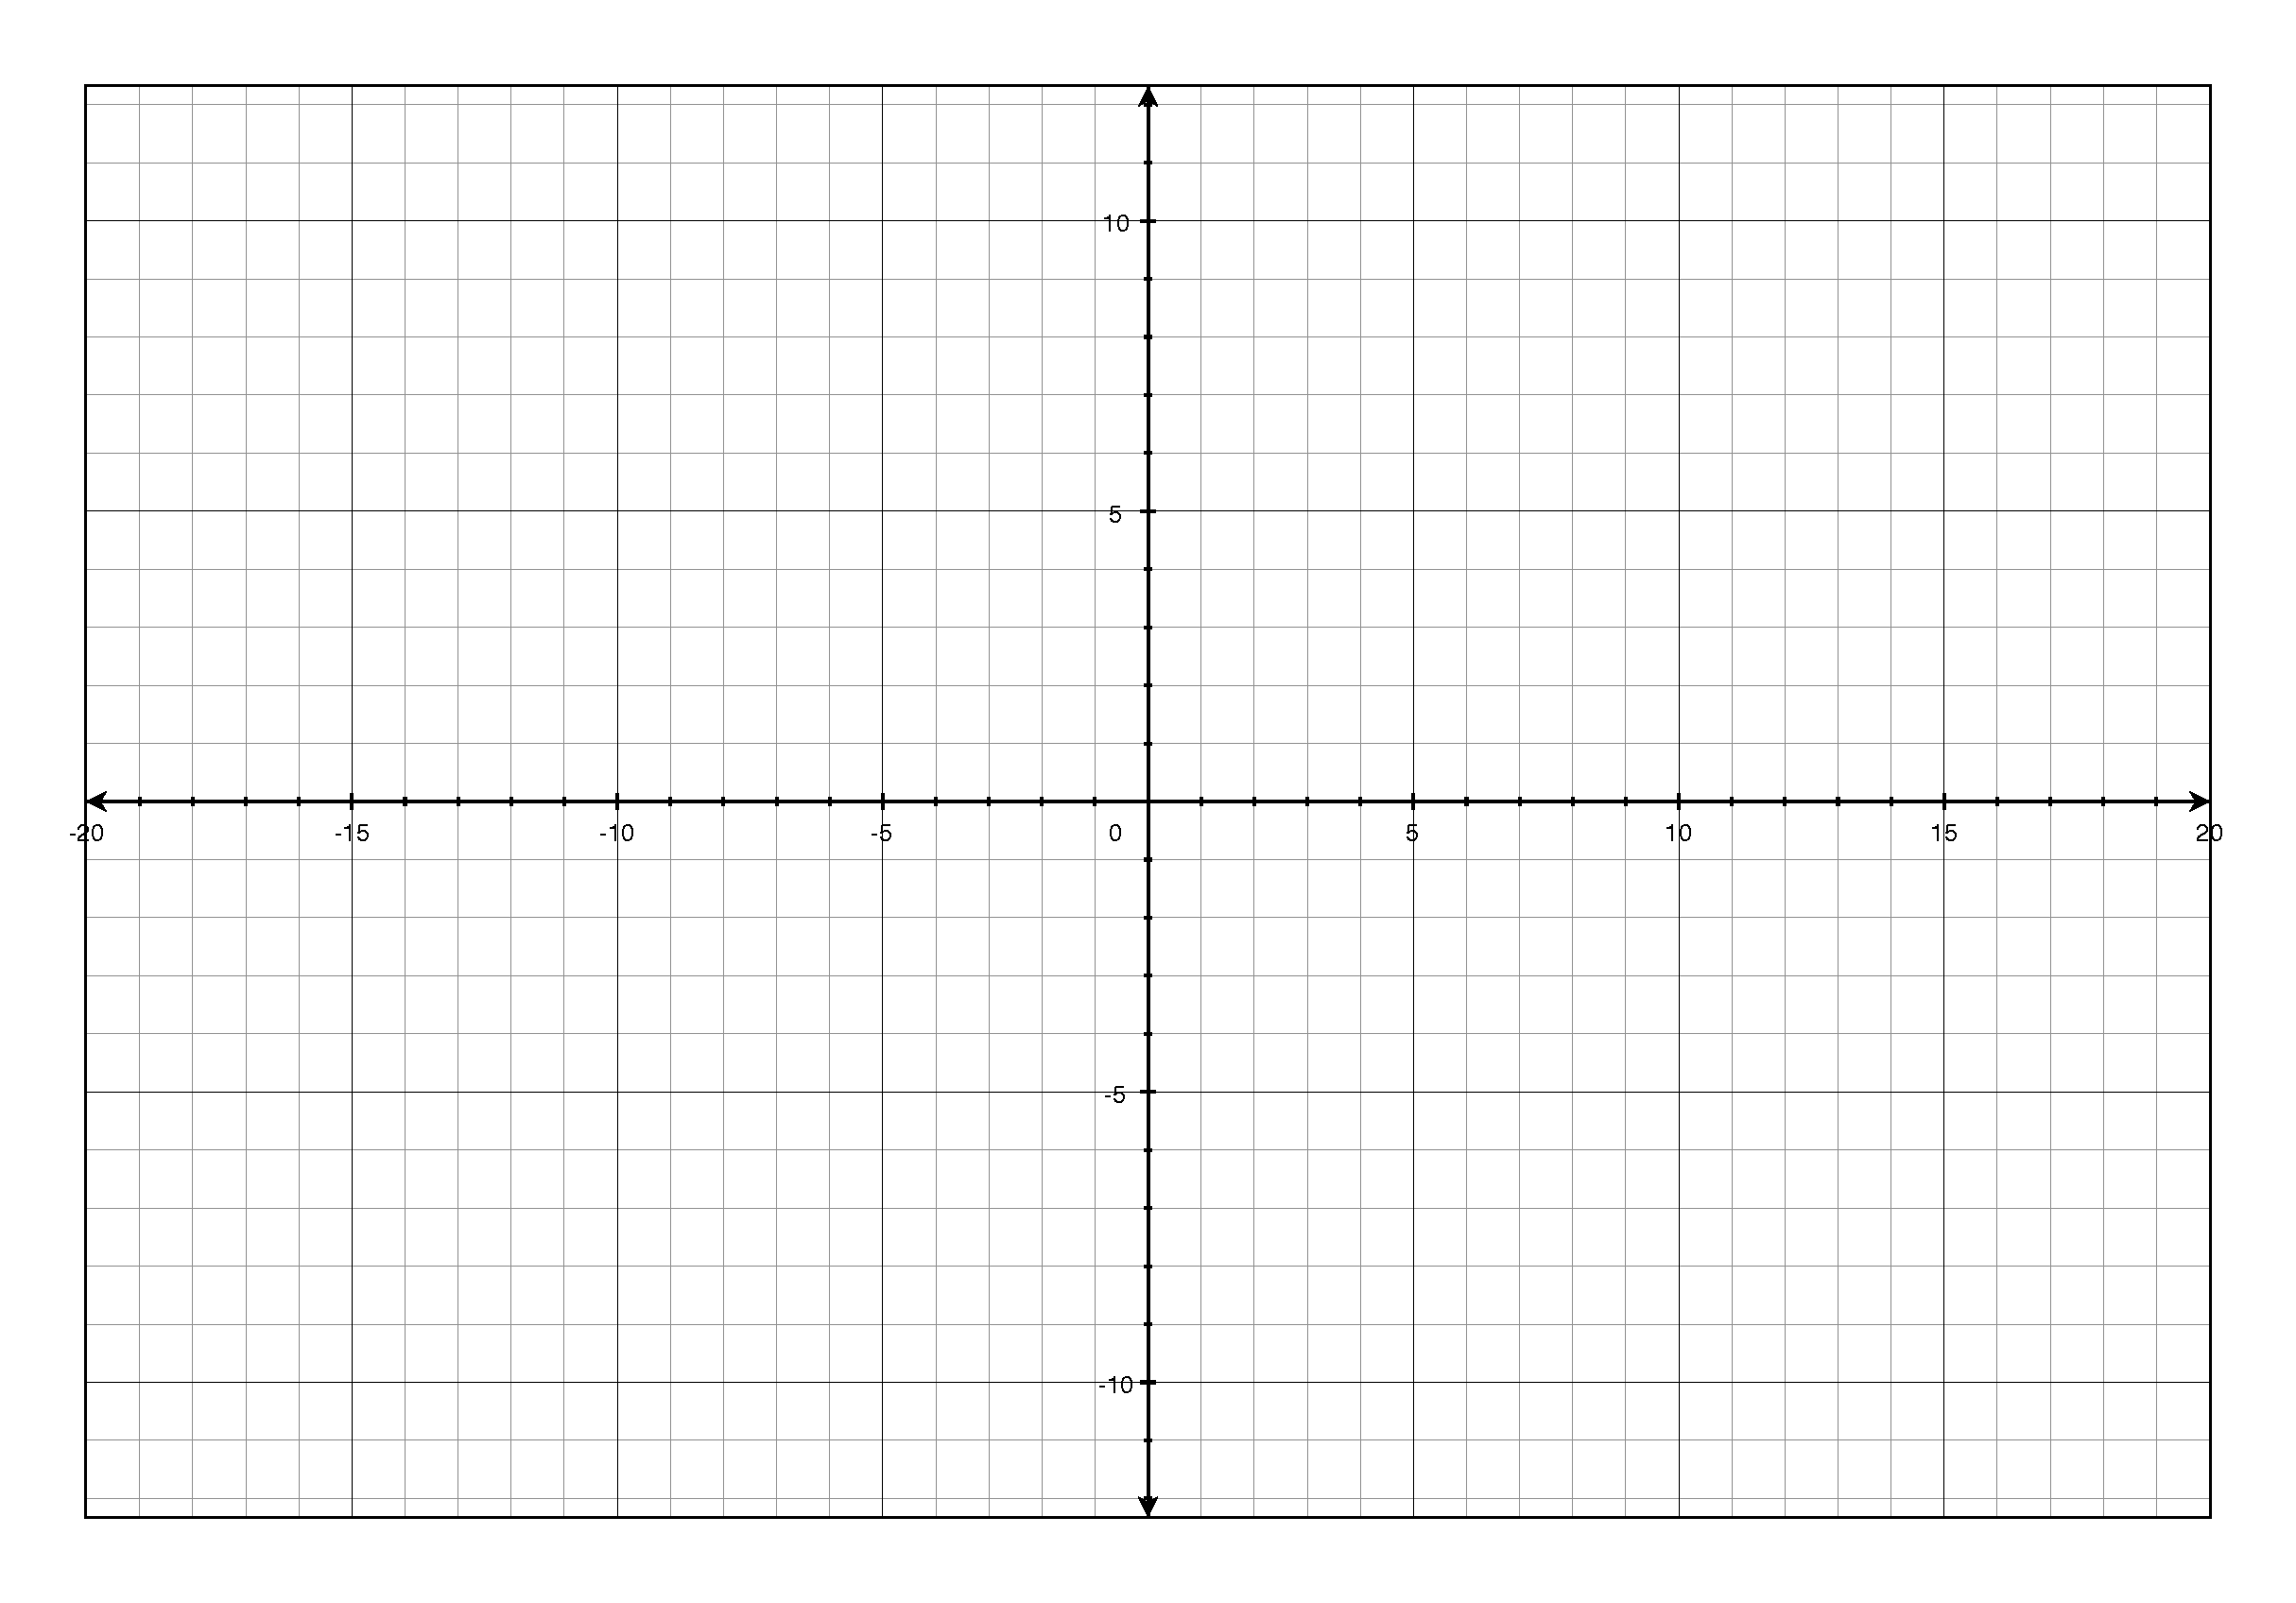
\includegraphics[width=15cm,height=9cm]{axes}
% \end{figure}

\question[5] \( y = - \dfrac{2}{3} x - 1\)

\label{graph:first}
\begin{figure}[H]
\ifprintanswers
  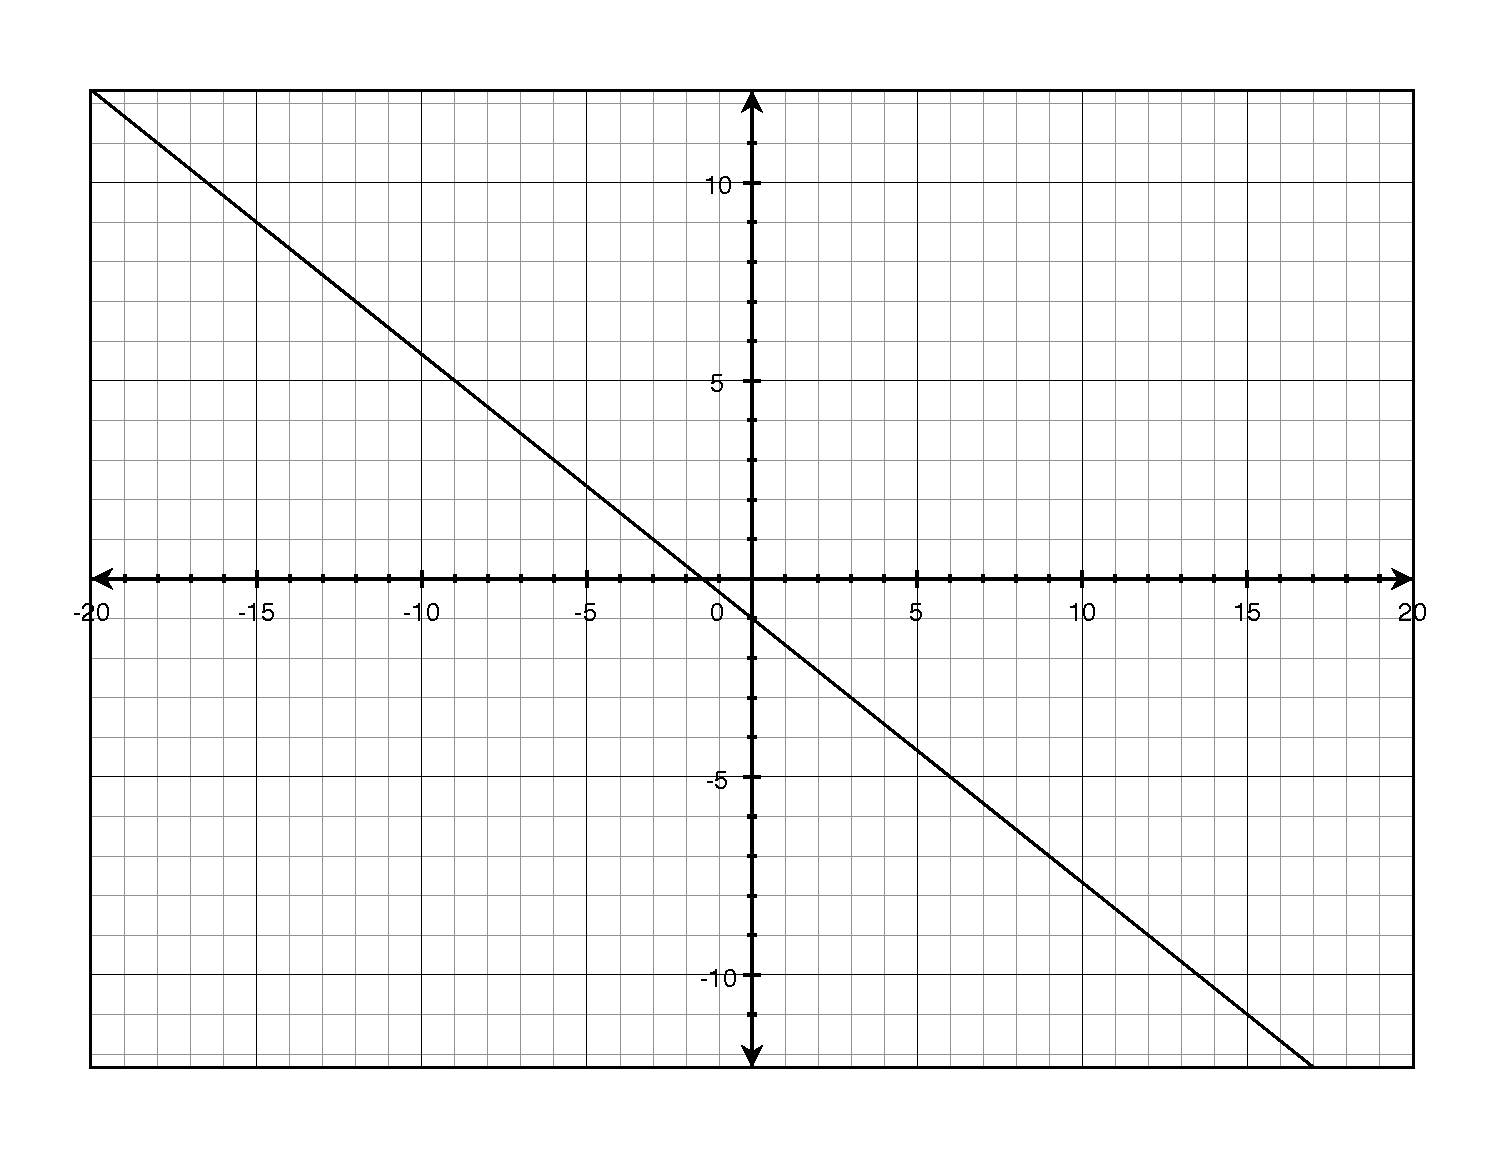
\includegraphics[width=12cm,height=7cm]{problem1}
\else
  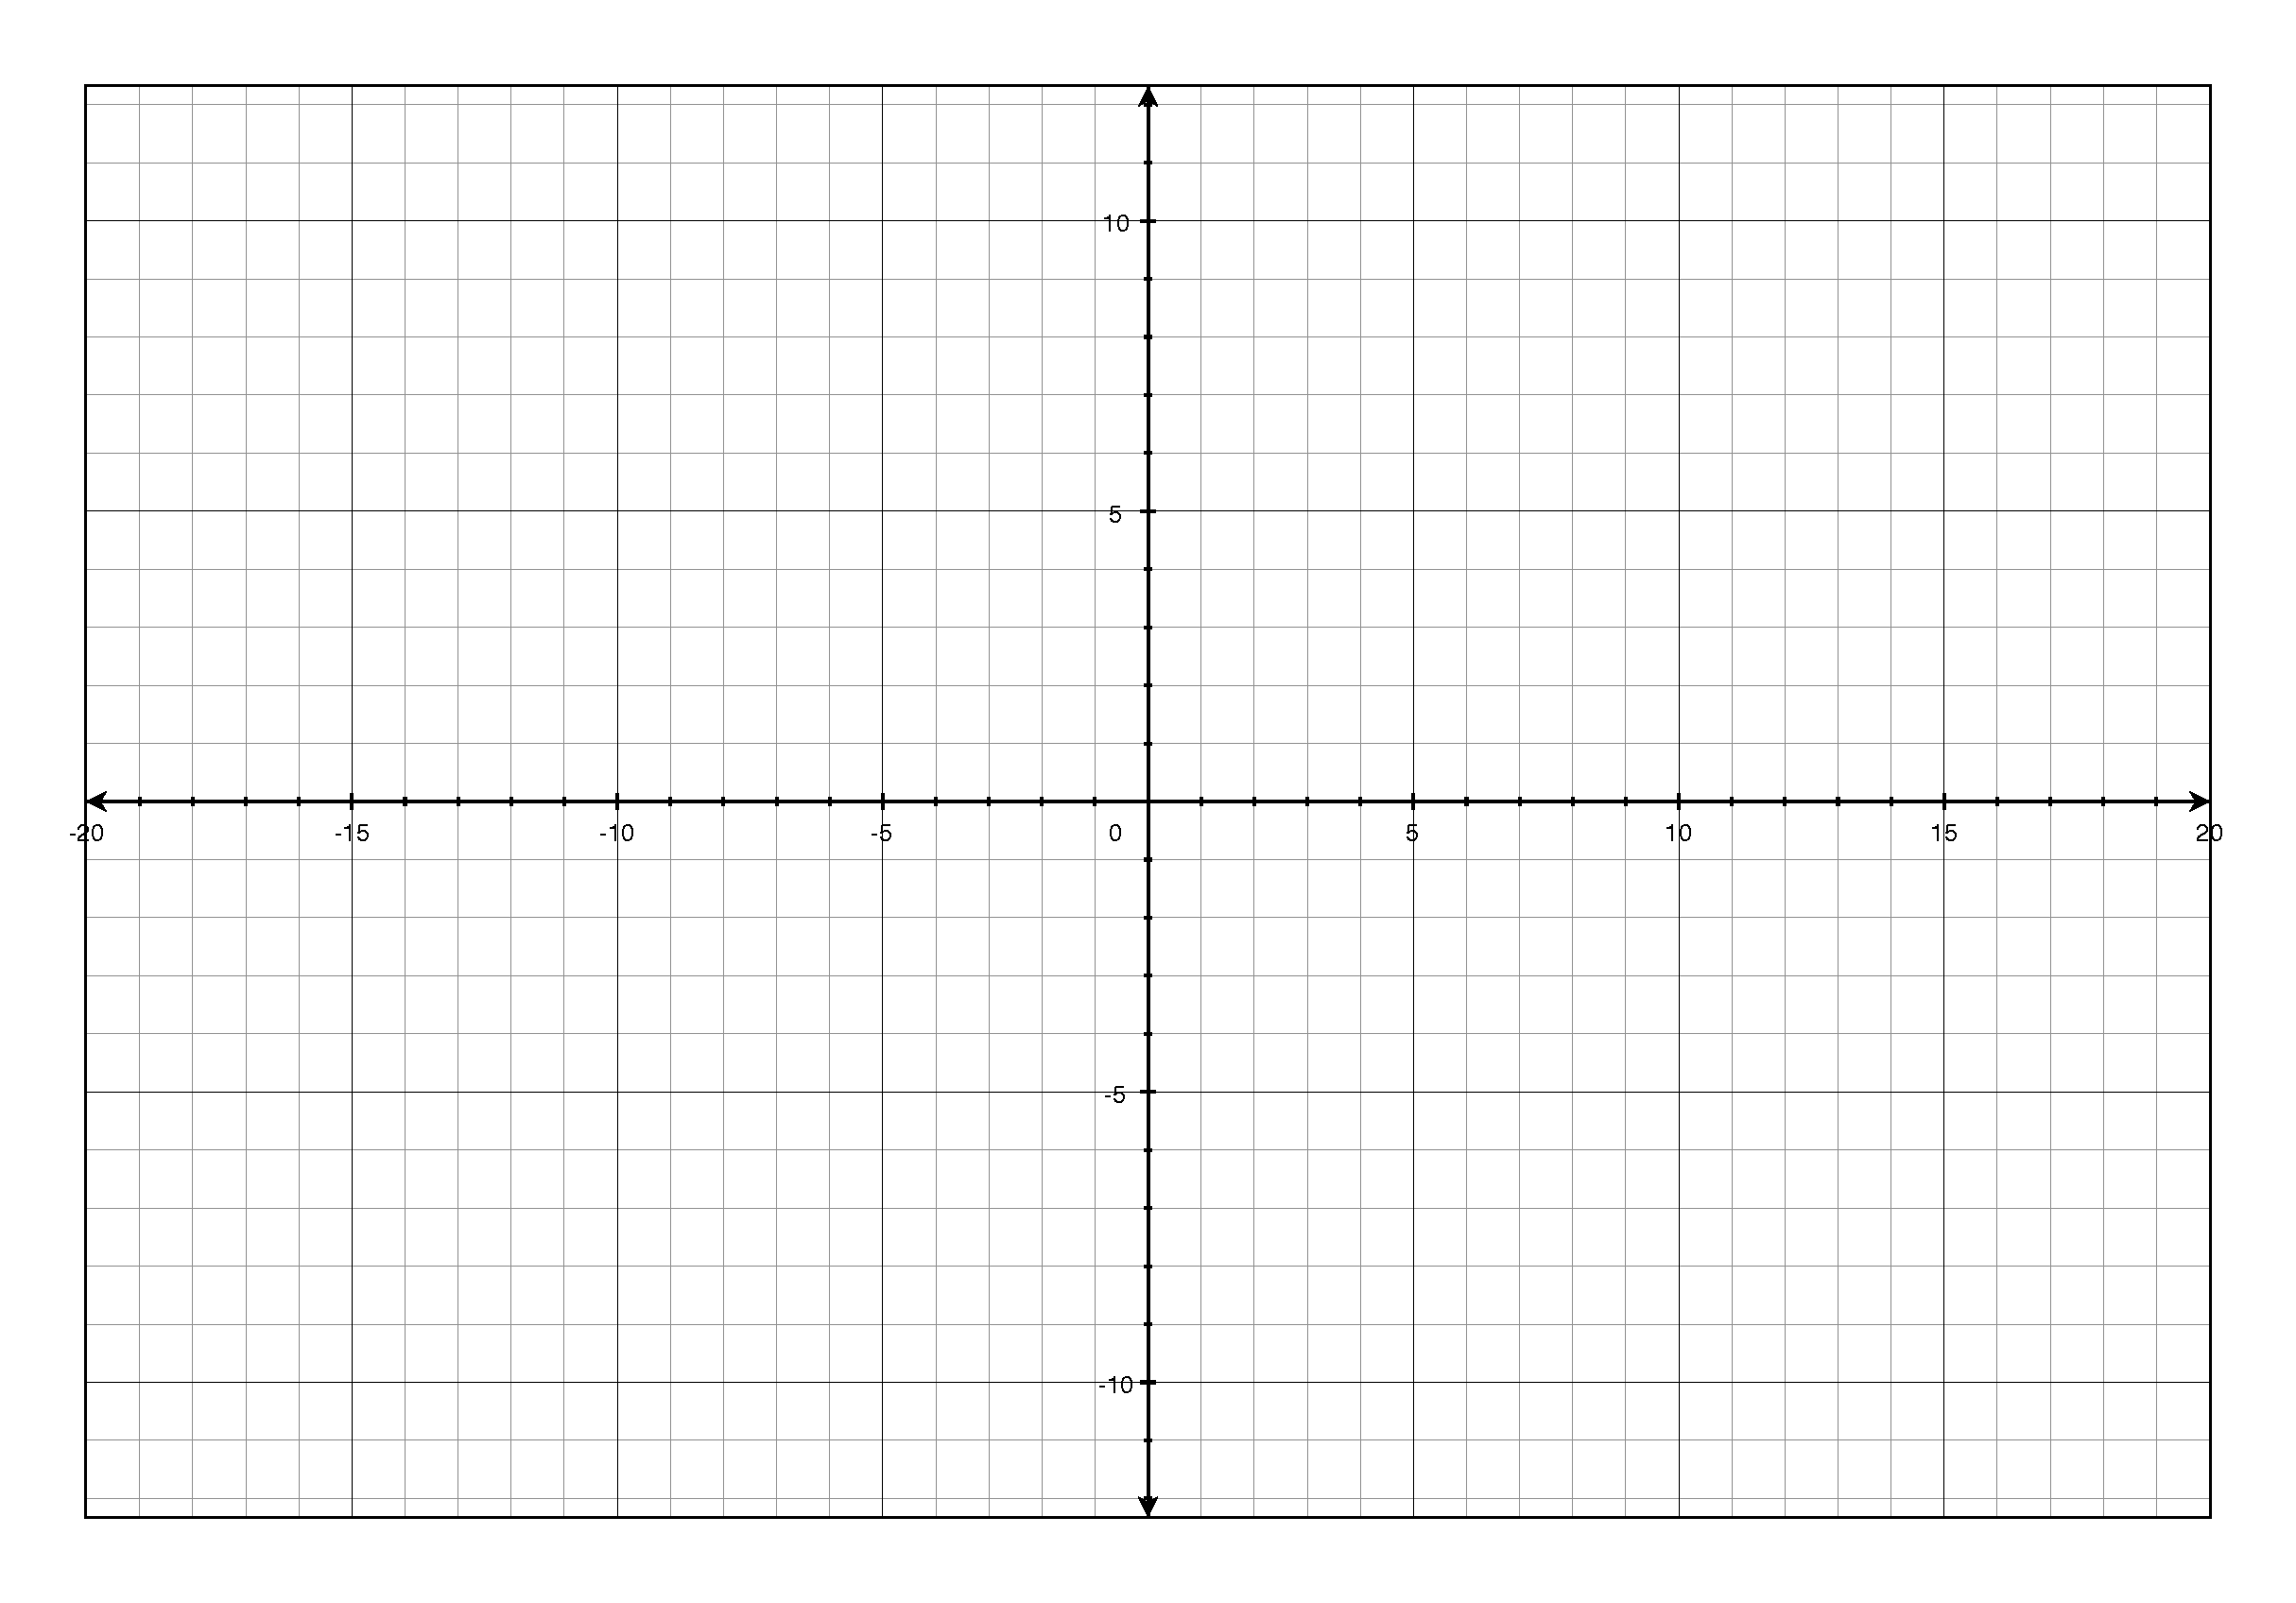
\includegraphics[width=15cm,height=9cm]{axes}
\fi
\end{figure}

\pagebreak

\question[5] \( x = 7\)
\begin{figure}[H]
\ifprintanswers
  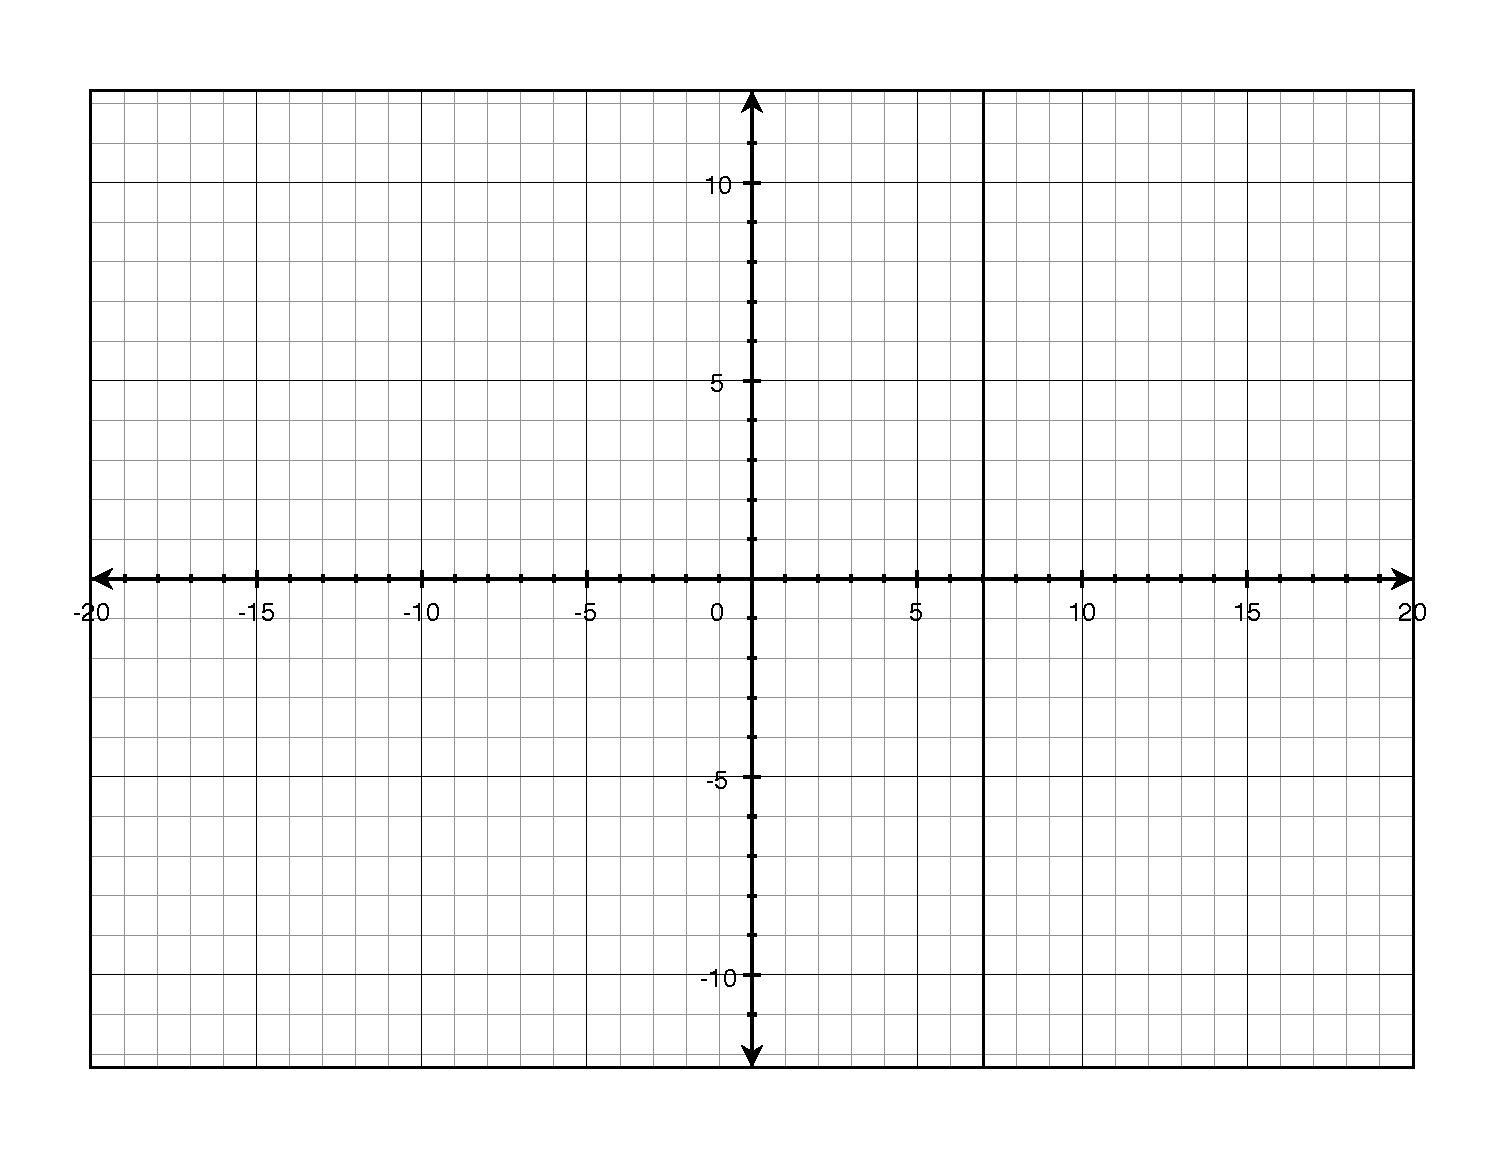
\includegraphics[width=12cm,height=7cm]{problem2}
\else
  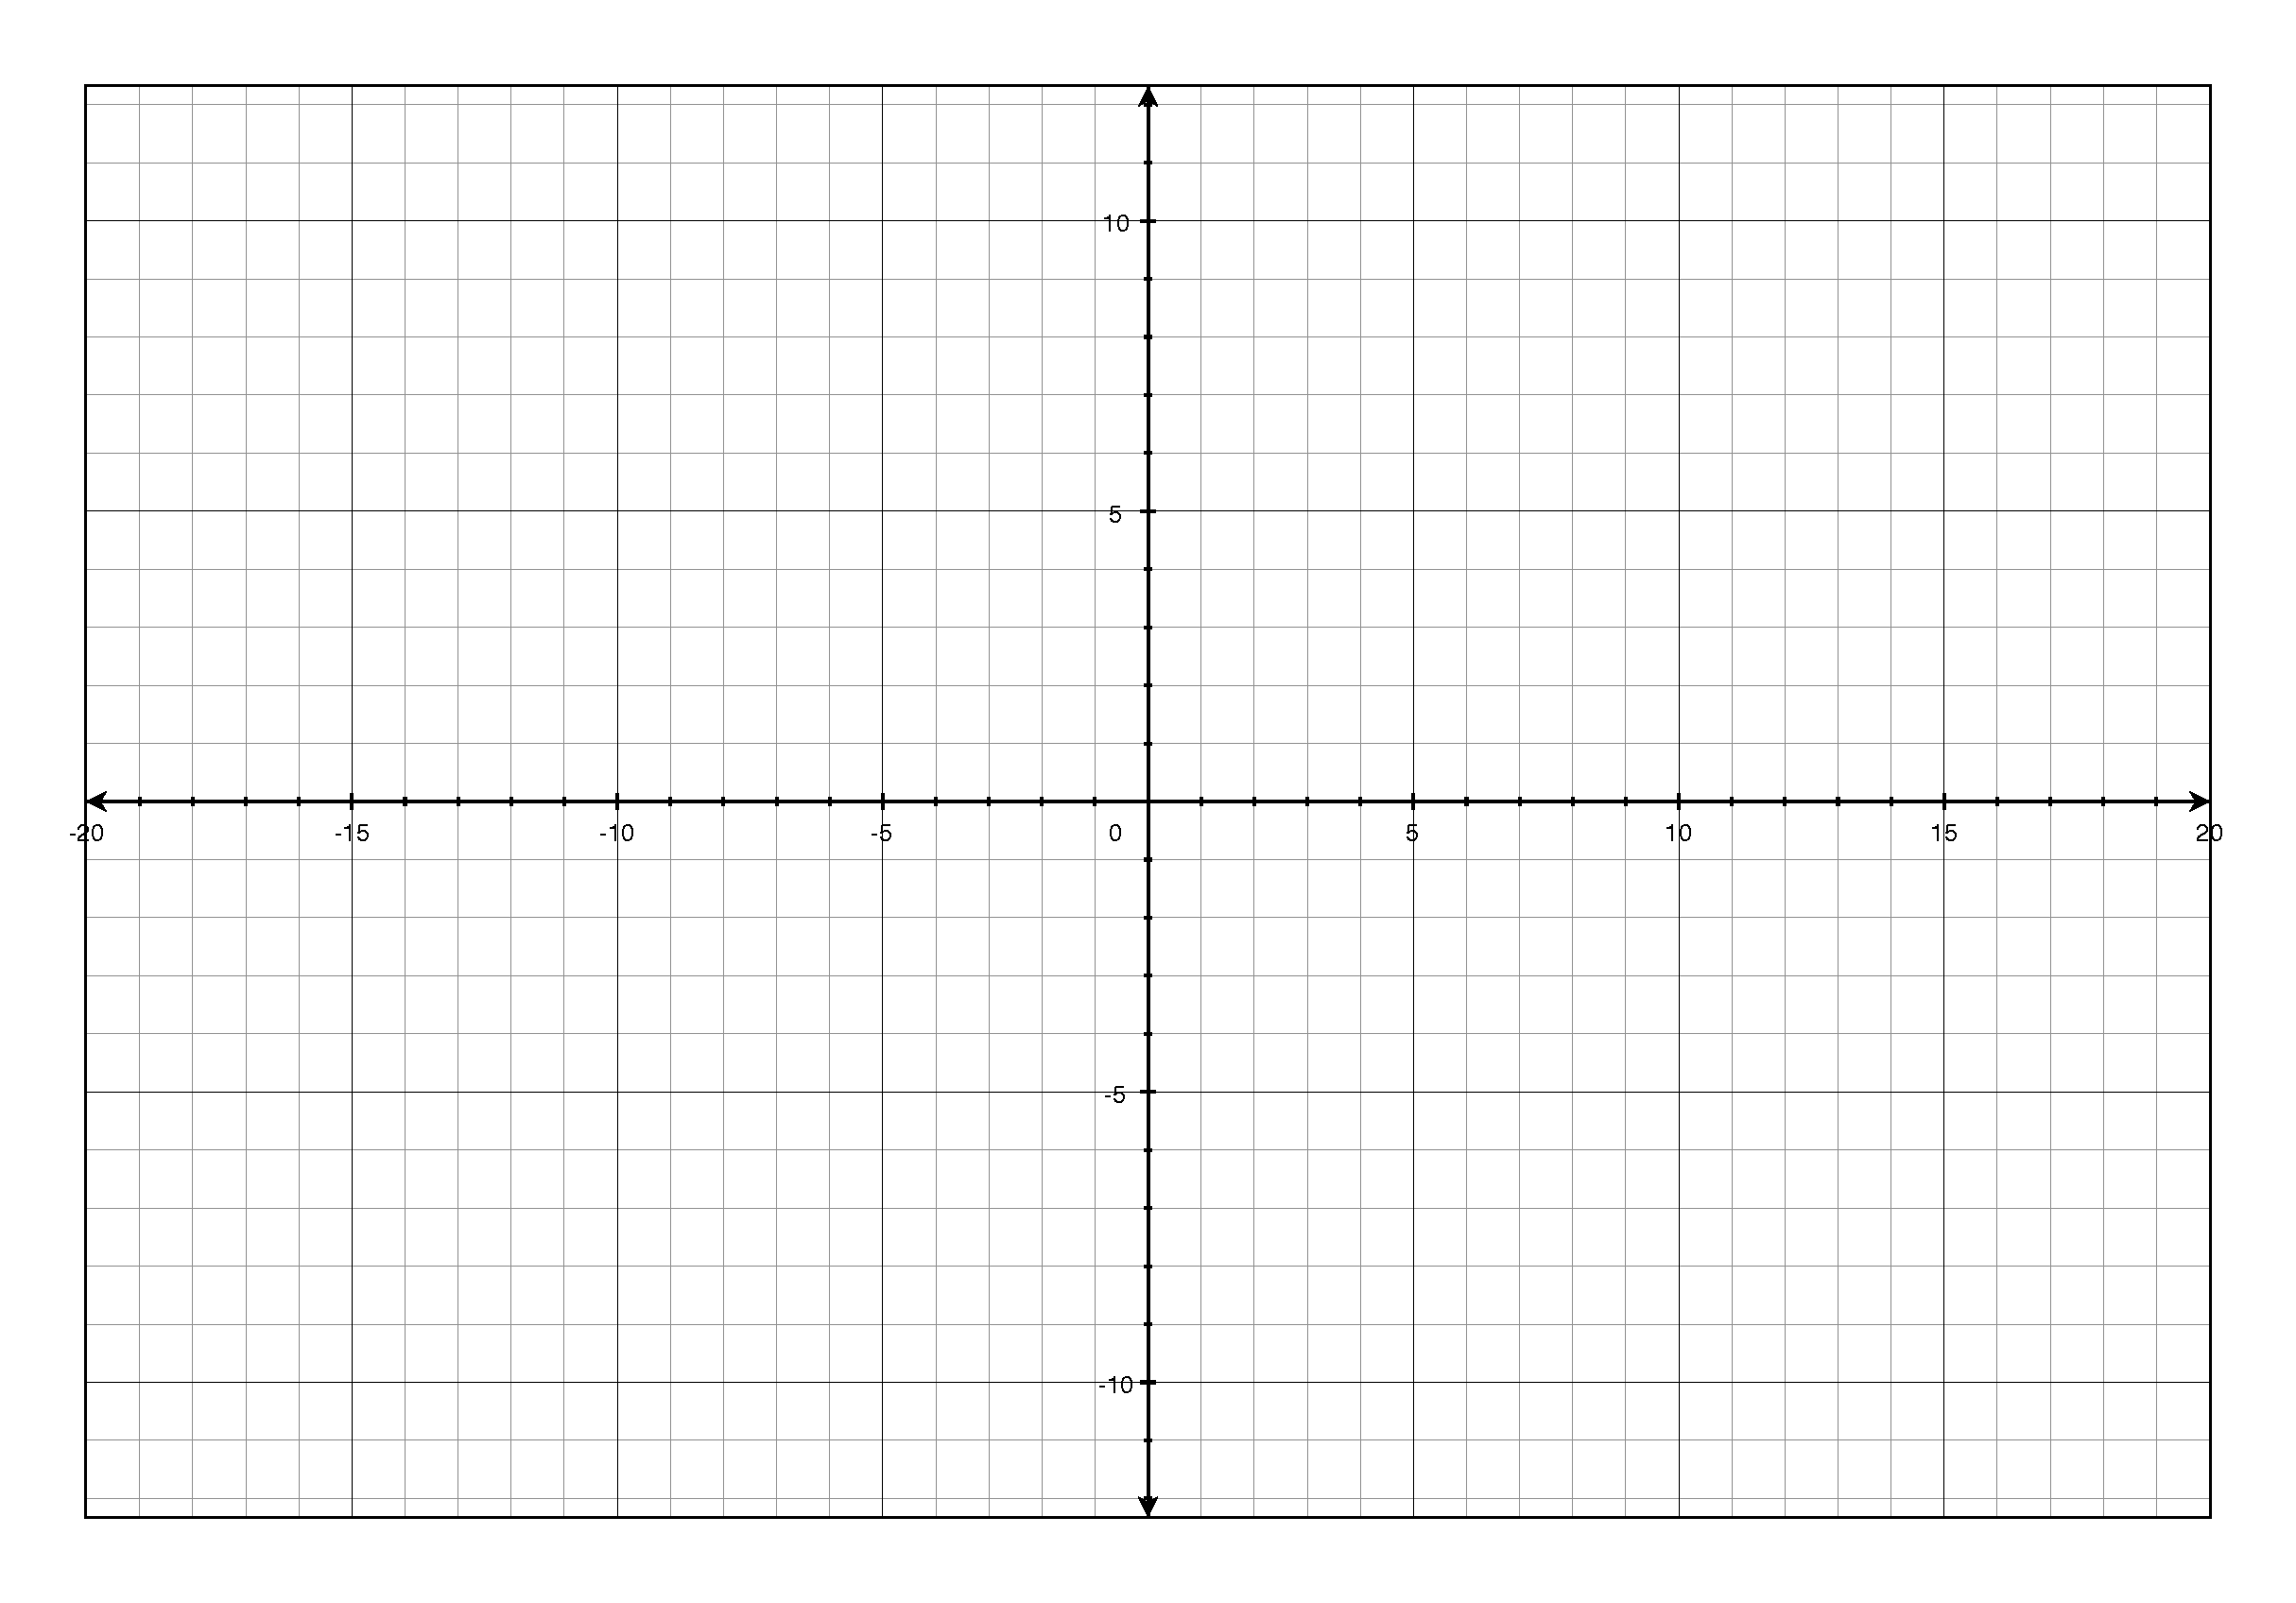
\includegraphics[width=15cm,height=9cm]{axes}
\fi
\end{figure}

\question[5] \( y = x^2 - 4\)
\label{graph:last}
\begin{figure}[H]
\ifprintanswers
  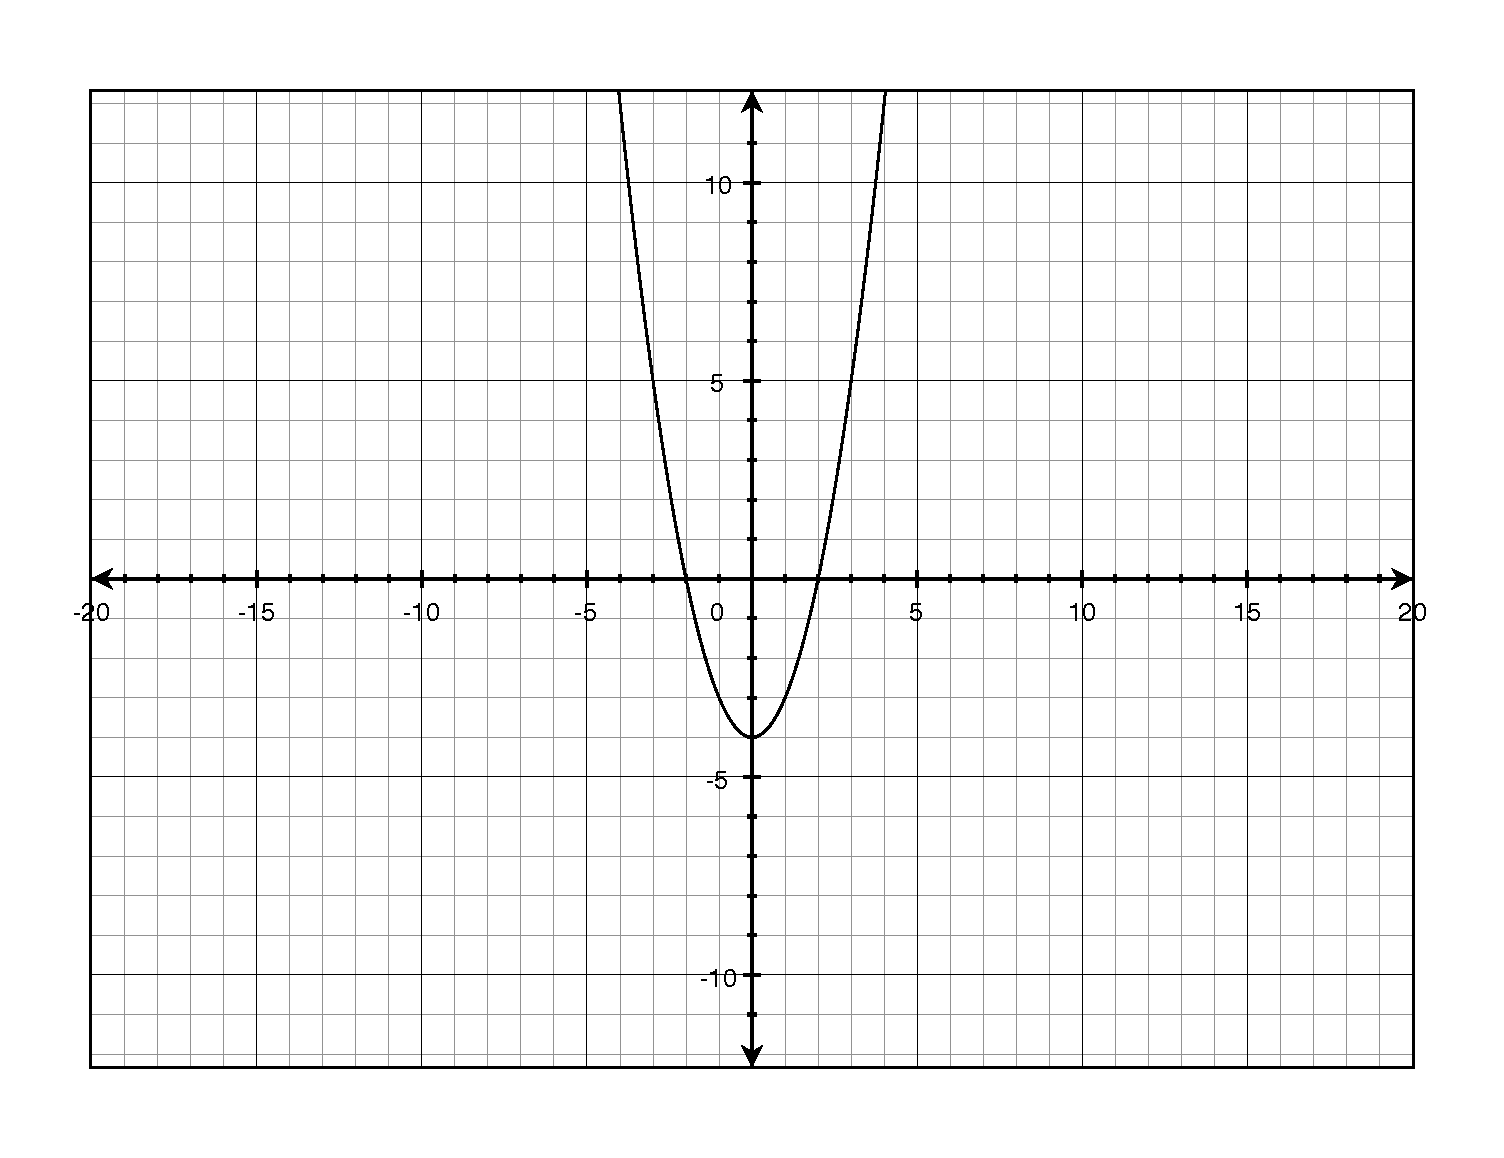
\includegraphics[width=12cm,height=7cm]{problem3}
\else
  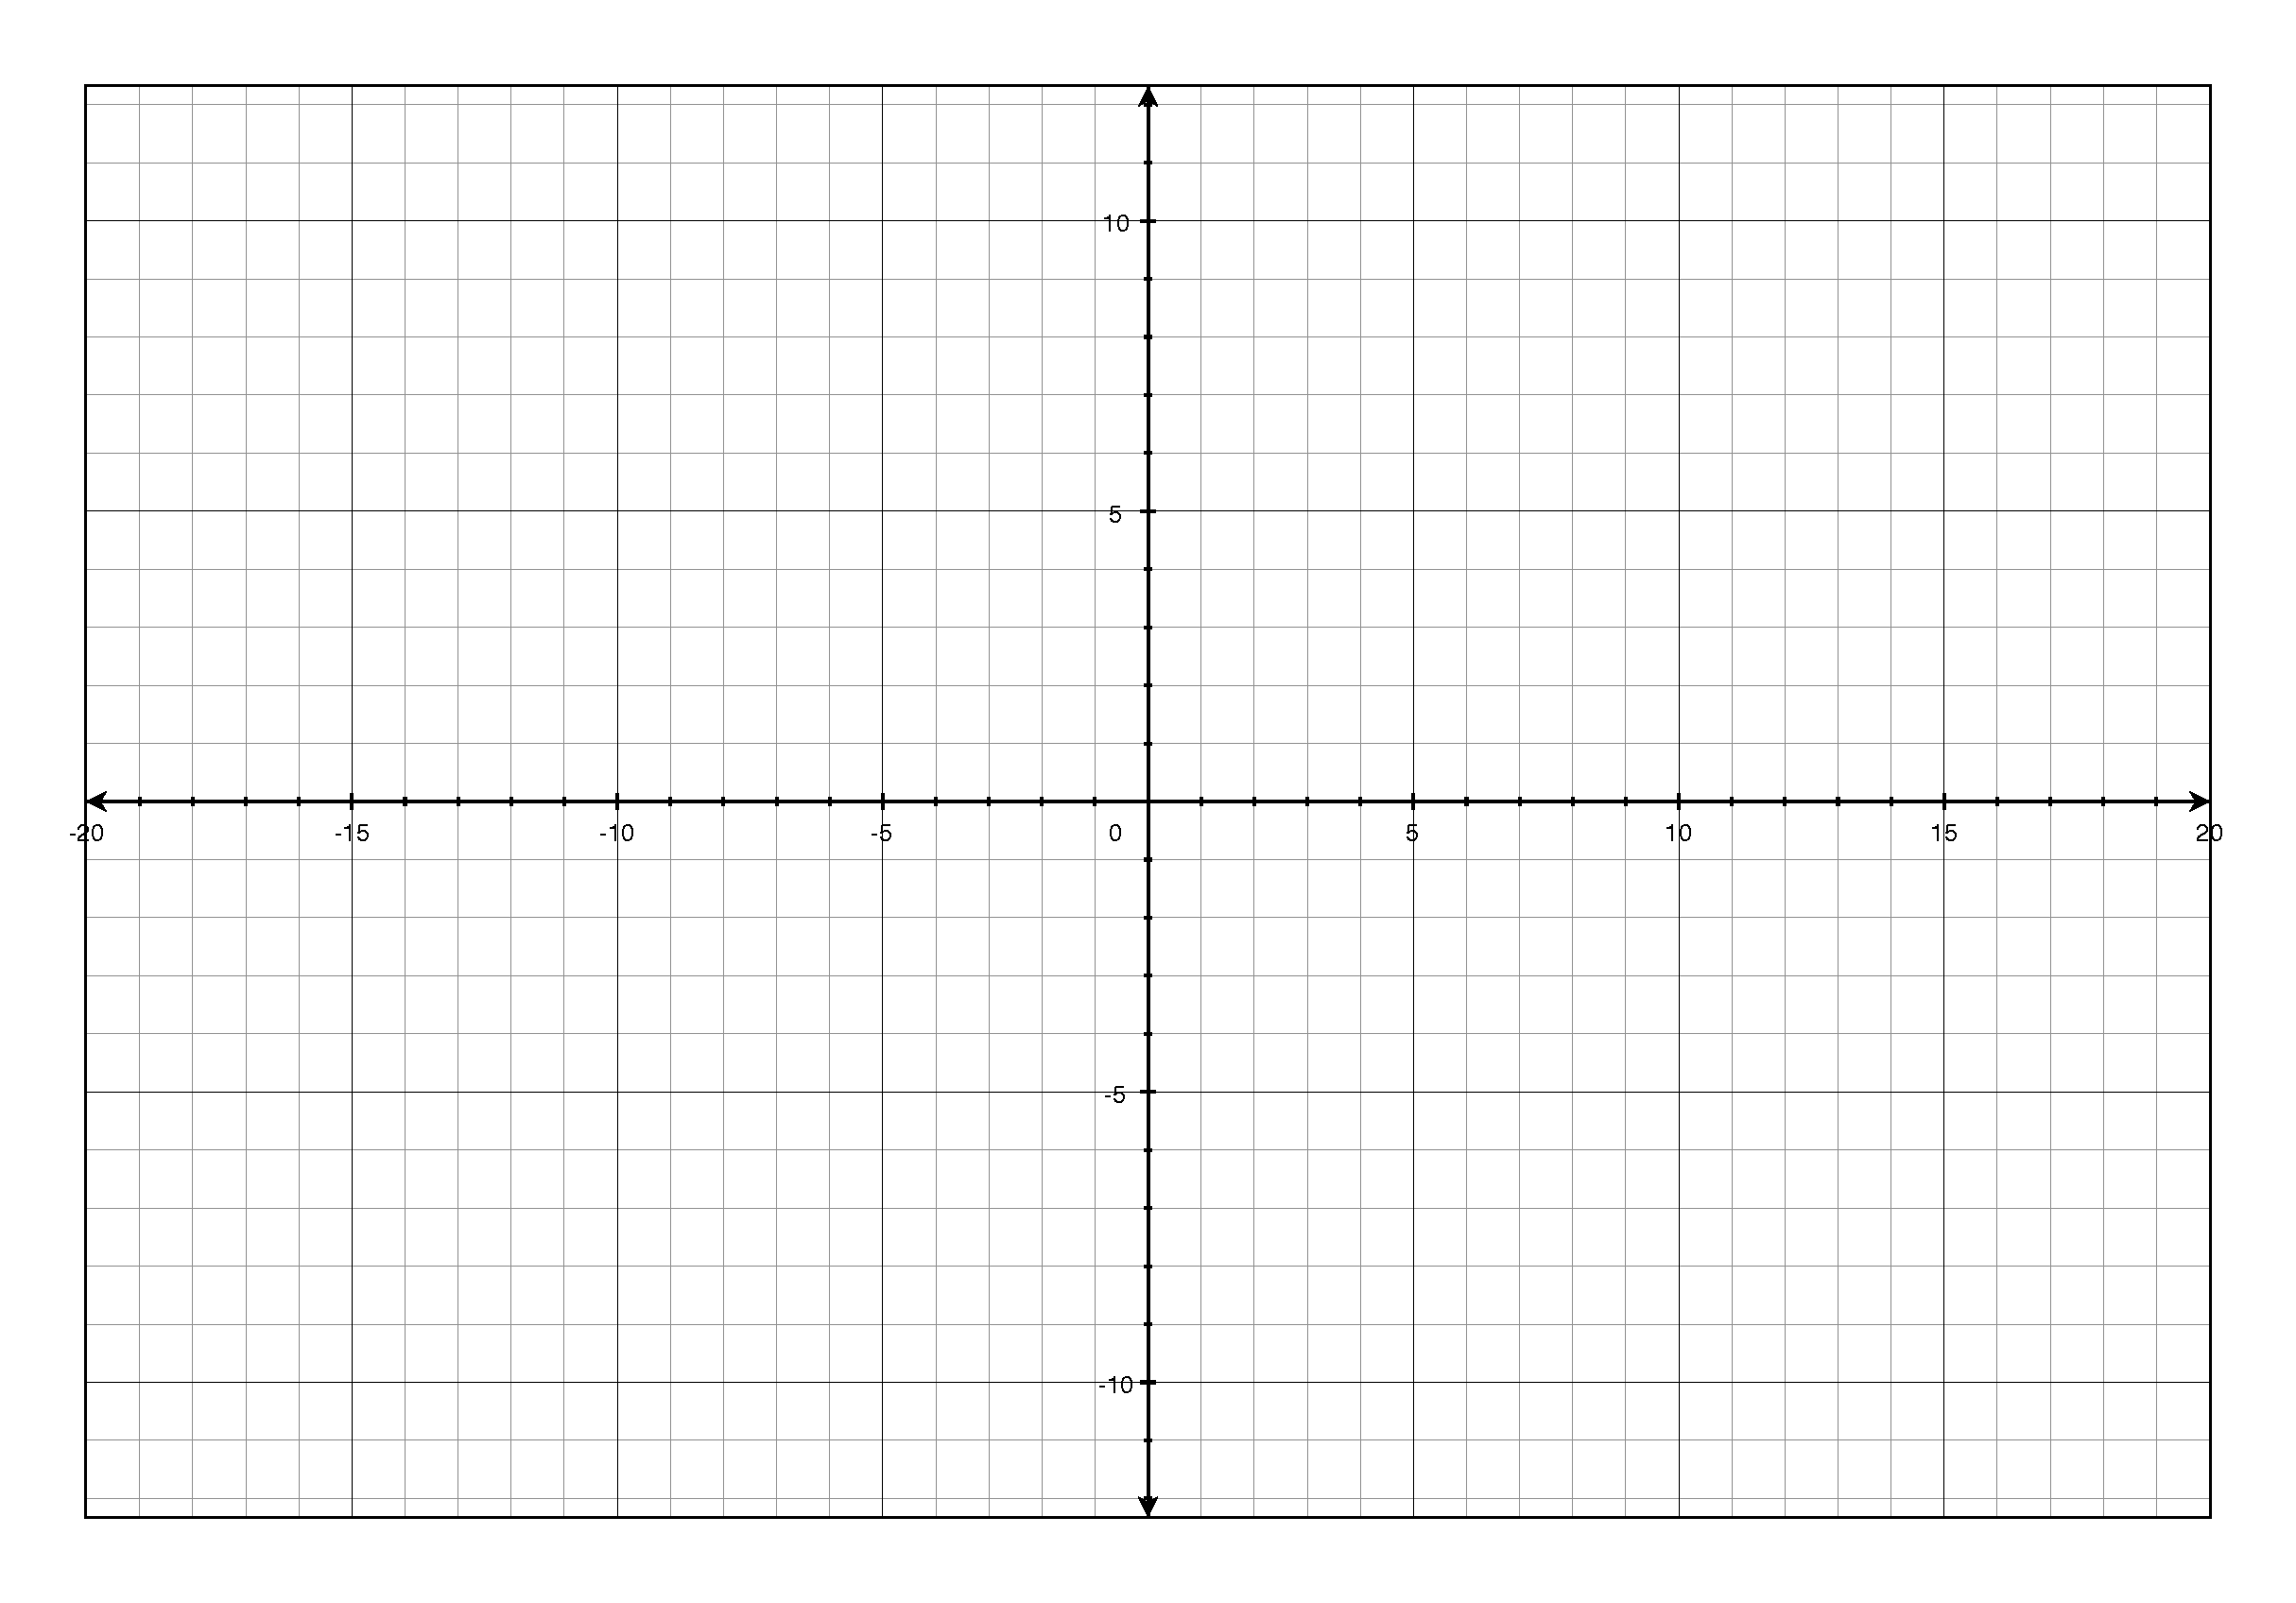
\includegraphics[width=15cm,height=9cm]{axes}
\fi
\end{figure}

\pagebreak

\question[5] \( y \geq \frac{1}{3} x + 4\)
\label{graph:last}
\begin{figure}[H]
\ifprintanswers
  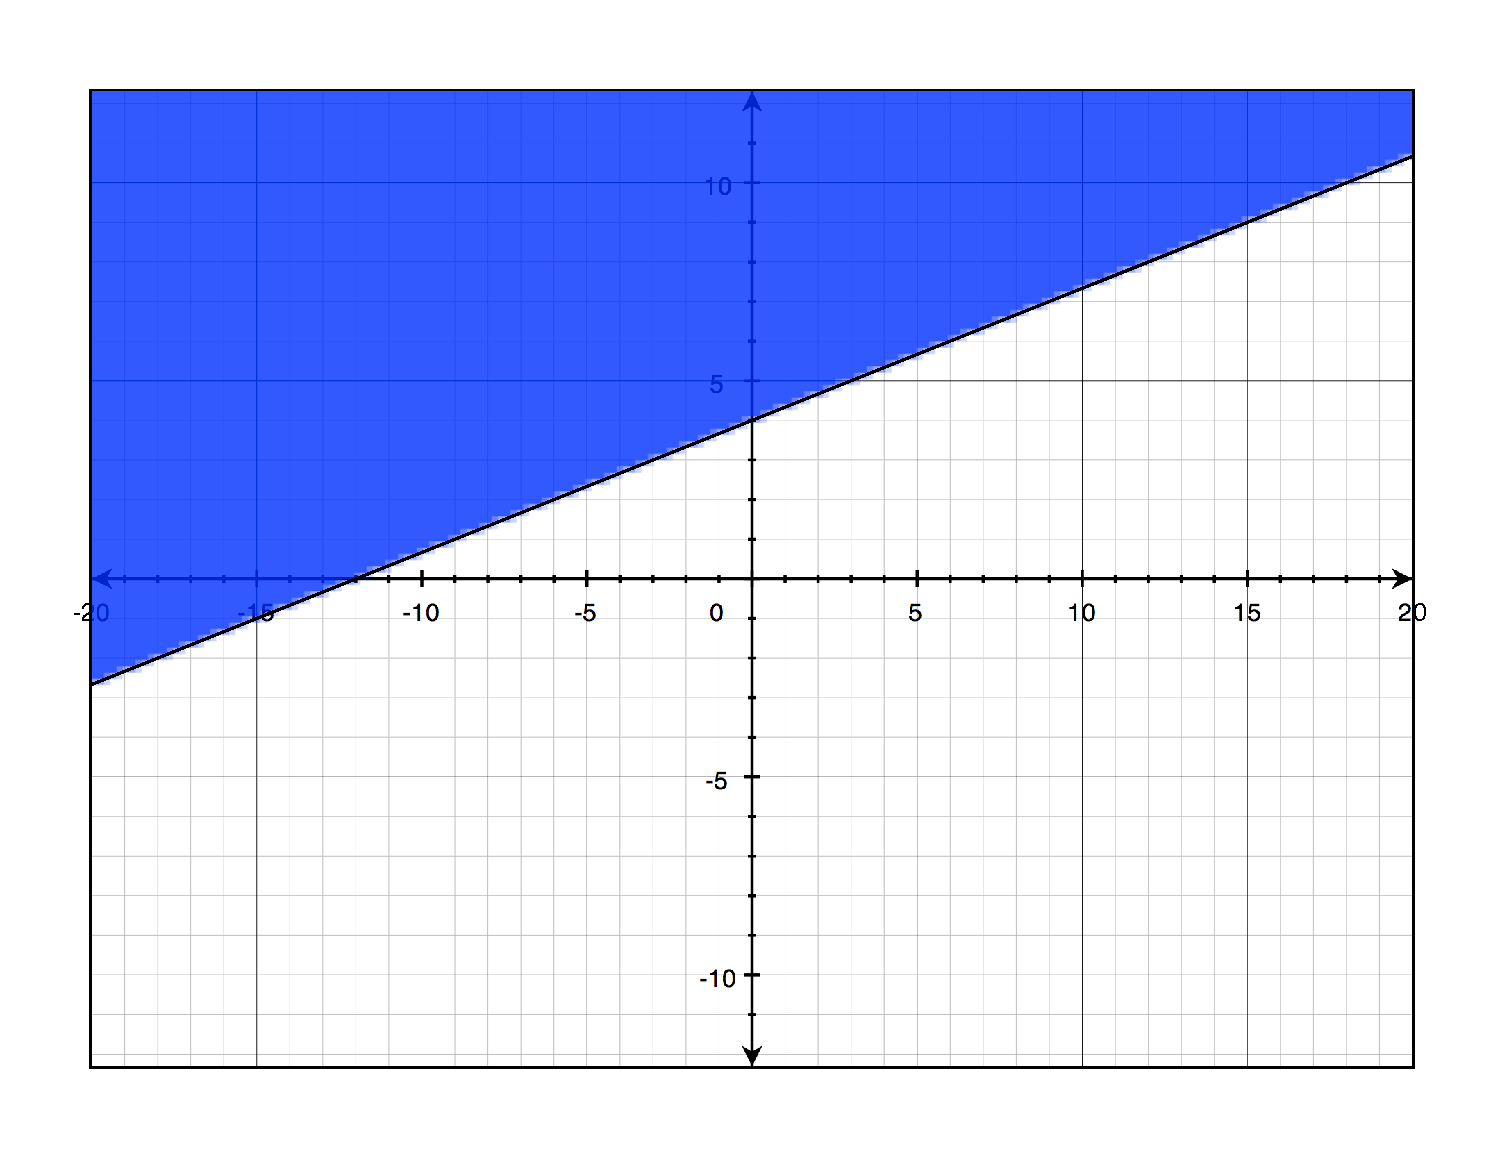
\includegraphics[width=12cm,height=7cm]{problem4}
\else
  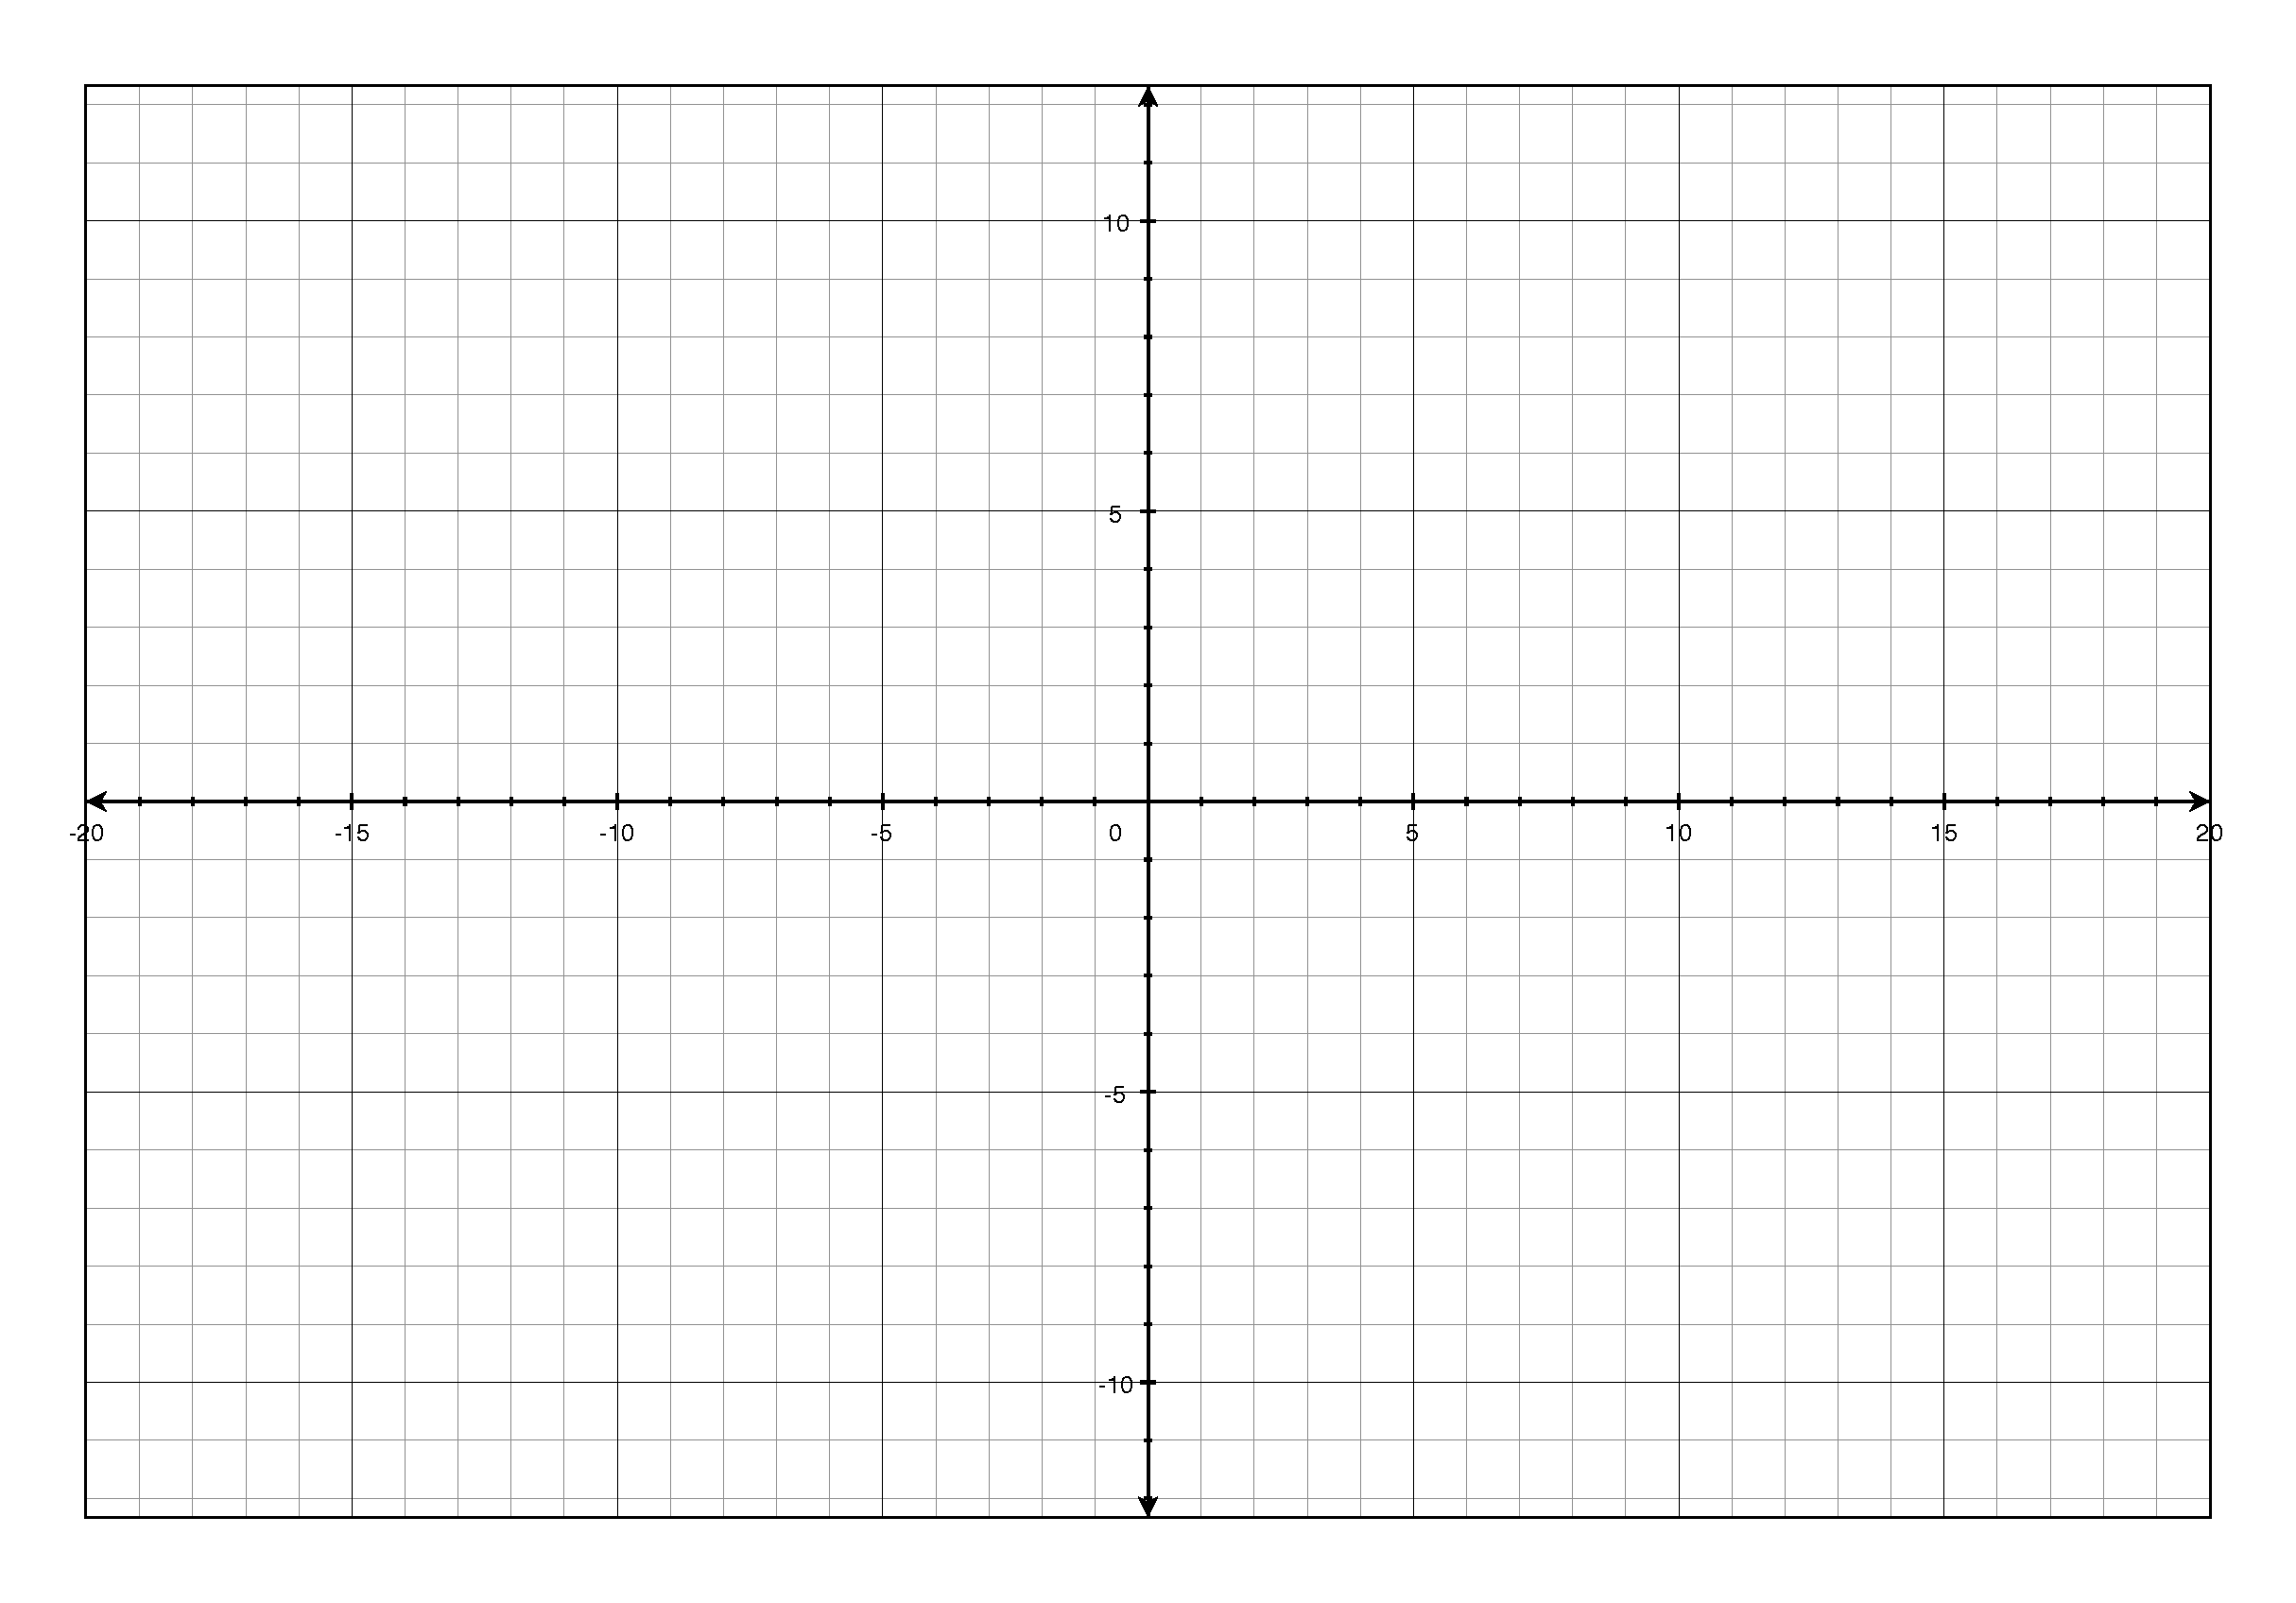
\includegraphics[width=15cm,height=9cm]{axes}
\fi

\end{figure}

\section{Distance}
For problems \ref{distance:first}-\ref{distance:last}, find the distance betwen each of the pairs of points.

\question[5] $(-2, 1)$ and $(3, 4)$
\label{distance:first}
\begin{solution}[4 cm]
\[
  d = \sqrt{(-2-3)^2 + (1-4)^2} = \sqrt{5^2 + 3^2} = \sqrt{34}
\]
\end{solution}

\question[5] $(3, 2)$ and $(-1, -6)$
\label{distance:last}
\begin{solution}[4 cm]
\[
  d = \sqrt{(-1-3)^2 + (-6-2)^2} = \sqrt{(-4)^2 + (-8)^2} = \sqrt{80} = 4\sqrt{5}
\]
\end{solution}

\ifprintanswers
\pagebreak
\fi

\section{Equations of Lines}

For problems \ref{equation:first}-\ref{equation:last}, find the equation of each line and express the final equation in standard form.

\question[10] $m=\dfrac{3}{4}$ containing $(4, -1)$
\label{equation:first}
\begin{solution}[6 cm]
\begin{align*}
  \frac{y - (-1)}{x - 4} &= \frac{3}{4} \\
  4y + 4 &= 3x - 12 \\
  3x - 4y &= 16 \\
\end{align*}

So the equation is: 
\begin{itemize}
  \item slope intercept form: $y = \dfrac{3}{4}x - 4$
  \item standard form: $3x-4y = 16$
\end{itemize}

% Find the y-intercept:

% \begin{align*}
%   y &= \frac{3}{4} x + b \\
%   -1 &= \frac{3}{4}(4) + b \\
%   -1 &= 3 + b \\
%   b &= -4
% \end{align*}


\end{solution}

\ifprintanswers
\pagebreak
\fi

\question[10] containing $(1, 2)$ and $(-3, 1)$
\begin{solution}[6 cm]

Find the slope:
\[
  m = \frac{1-2}{-3-1} = \frac{-1}{-4} = \frac{1}{4}
\]

Use one of the points to find the equation:
\begin{align*}
  \frac{1}{4} &= \frac{1-y}{-3-x} \\
  -3-x &= 4 - 4y \\
  -4y &= -x-7 \\
  y &= \frac{1}{4} x + \frac{7}{4} \\
\end{align*}

So the equation is: 
\begin{itemize}
  \item slope intercept form: $y = \frac{1}{4} x + \frac{7}{4}$
  \item standard form: $x-4y = -7$
\end{itemize}

\end{solution}

\question[10] containing $(3, 7)$ and perpendicular to $y = -\dfrac{1}{3} x + 4$
\label{equation:last}
\begin{solution}[6 cm]
The slope of the perpendicular line is the negative reciprocal, or $3$.

\begin{align*}
  3 &= \frac{y-7}{x-3} \\
  3(x-3) &= y-7 \\
  3x-9 &= y-7 \\
  y &= 3x-2 \\
\end{align*}

So the equation is: 
\begin{itemize}
  \item slope intercept form: $y = 3x - 2$
  \item standard form: $3x - y = 2$
\end{itemize}

\end{solution}

\ifprintanswers
\else
\pagebreak
\fi

\section{Systems of Equations}
For problems \ref{system:first}-\ref{system:last}, solve each system of equations using any method.

\question[10] 
\label{system:first}
\begin{align*}
  2x - 3y &= -7 \\
  3x + y &= -5 \\
\end{align*}

\begin{solution}[6 cm]
Solve the second equation for $y$: $y = -3x - 5$

Substitute:
\begin{align*}
  2x - 3(-3x - 5) &= -7 \\
  2x + 9x + 15 &= -7 \\
  11x &= -22 \\
  x &= -2
\end{align*}

Find $y$: $y = -3(-2) - 5 = 6-5 = 1$

So the solution is: (-2, 1)

\end{solution}

\ifprintanswers
\pagebreak
\fi

\question[10] 
\begin{align*}
  5x + 3y &= 6 \\
  2x - 4y &= 5 \\
\end{align*}

\begin{solution}[8 cm]
\begin{align*}
  5x + 3y &= 6 \\
  2x - 4y &= 5 \\
  \\
  -10x - 6y &= -12 \\
  10x - 20y &= 25 \\
  \\
  -26y &= 13 \\
  y &= - \frac{1}{2} \\
\end{align*}

Find $x$: 

\begin{align*}
  2x - 4(- \frac{1}{2}) &= 5 \\
  2x + 2 &= 5 \\
  2x &= 3 \\
  x &= \frac{3}{2}
\end{align*}

So the solution is: $\left( \dfrac{3}{2}, - \dfrac{1}{2} \right)$

\end{solution}

% \question[10] 
% \begin{align*}
%   4y - 2x &= 9 \\
%   6y - 3x &= -2 \\
% \end{align*}

% \begin{solution}[4 cm]
% no solution
% \end{solution}

\ifprintanswers
\else
\pagebreak
\fi

\question[10] 
\begin{align*}
  \frac{x}{3} - \frac{y}{5} &= 1 \\
  \frac{x}{12} + \frac{y}{40} &= 1 \\
\end{align*}

\begin{solution}[6 cm]
\begin{align*}
  \frac{x}{3} - \frac{y}{5} &= 1 \\
  \frac{x}{12} + \frac{y}{40} &= 1 \\
  \\
  5x - 3y &= 15 \\
  10x + 3y &= 120 \\
  \\
  5x - 3y &= 15 \\
  15x &= 135 \\
  \\
  5x - 3y &= 15 \\
  x &= 9 \\
\end{align*}

Find $y$:
\begin{align*}
  \frac{9}{3} - \frac{y}{5} &= 1 \\
  3 - \frac{y}{5} &= 1 \\
  15 - y &= 5 \\
  y &= 10 \\
\end{align*}

So the solution is: $(9, 10)$
\end{solution}

% \question[15] 
% \label{system:last}
% \begin{align*}
%   x - 2y + 2z &= 9 \\
%   -x + 3y &= -4 \\
%   2x - 5y + z &= 10 \\
% \end{align*}

% \begin{solution}[10 cm]
% $(1, -1, 3)$
% \end{solution}

\question[15] 
\label{system:last}
\begin{align*}
  4x + y -3z &= 11 \\
  2x - 3y + 2z &= 9 \\
  x + y + z &= -3 \\
\end{align*}

\begin{solution}[8 cm]
\begin{align*}
  4x + y -3z &= 11 \\
  2x - 3y + 2z &= 9 \\
  x + y + z &= -3 \\
\end{align*}

Use the third equation to get rid of $y$ in the other two:
\begin{align*}
  4x + y -3z &= 11 \\
  2x - 3y + 2z &= 9 \\
  x + y + z &= -3 \\  
  \\
  x + y + z &= -3 \\  
  -3y - 7z &= 23 \\
  2x - 3y + 2z &= 9 \\  
  \\
  x + y + z &= -3 \\  
  -3y - 7z &= 23 \\
  -5y      &= 15 \\
  \\
  x + y + z &= -3 \\  
  -3y - 7z &= 23 \\
  y      &= -3 \\
\end{align*}

Find $z$: 
\begin{align*}
  -3y - 7z &= 23 \\
  -3(-3) - 7z &= 23 \\
  9 - 7z &= 23 \\
  -7z &= 14 \\
  z &= -2 \\
\end{align*}

Find $x$:
\begin{align*}
  x + (-3) + (-2) &= -3 \\  
  x - 5 &= -3 \\  
  x  &= 2 \\  
\end{align*}

So the solution is: $(2, -3, -2)$
\end{solution}

\ifprintanswers
\pagebreak
\fi

\section{Word Problems}
\question[10] 
Widgets, Inc. makes both gadgets and widgets.  Widgets sell for \$5 and gadgets sell for \$10.  If 30 items sold for
\$230, how many of each type of item was sold?

\begin{solution}[8 cm]
Let:
\begin{description}
  \item[g] be the number of gadgets
  \item[w] be the number of widgets
\end{description}

The two equations are:
\begin{align*}
  g + w &= 30 \\
  10g + 5w &= 230
\end{align*}

Solve the first equation for $w$: $w = 30 - g$.

Substitute:
\begin{align*}
  10g + 5(30 - g) &= 230 \\
  10g + 150 - 5g &= 230 \\
  5g + 150 &= 230 \\
  5g  &= 80 \\
  g &= 16 \\
\end{align*}

So $w = 30 - 16 = 14$

Check: $10 \cdot 16 + 5 \cdot 14 = 160 + 70 = 230$

\end{solution}

\question[15] 
The performance of a play made \$540 on the first night and \$850 on the second night.  There are student tickets
and general admission tickets.  On the first night there were 150 student tickets and 80 general admission tickets.  On
the second night, there were 200 student tickets and 150 general admission tickets.  What is the price of each type of
ticket?

\begin{solution}[8 cm]
Let:
\begin{description}
  \item[x] be the student ticket price
  \item[y] be the general admission ticket price
\end{description}

The two equations are:
\begin{align*}
  150x + 80y &= 540 \\
  200x + 150y &= 850 \\
\end{align*}

Simplify the equations by making the numbers a little smaller:
\begin{align*}
  150x + 80y &= 540 \\
  200x + 150y &= 850 \\
  \\
  15x + 8y &= 54 \\
  20x + 15y &= 85 \\
  \\
  15x + 8y &= 54 \\
  4x + 3y &= 17 \\
\end{align*}

Solve the second equation for $y$:
\begin{align*}
  4x + 3y &= 17 \\
 3y &= 17 - 4x\\
 y  &= \frac{17 - 4x}{3} \\
\end{align*}

Subsititute:
\begin{align*}
  15x + 8y &= 54 \\
  15x + 8 \left( \frac{17 - 4x}{3} \right) &= 54 \\
  45x + 8(17-4x) &= 162 \\
  45x + 136 -32x &= 162 \\
  13x + &= 26 \\
  x &= 2 \\
\end{align*}

Find $y$: $y = \dfrac{17 - 4x}{3} = \dfrac{17 - 4(2)}{3} = \dfrac{9}{3} = 3$

So the student price is \$2 and the general admission price is \$3.

check: 
\begin{itemize}
  \item on the first night they made: $150 \cdot 2 + 80 \cdot 3 = 540$
  \item on the second night they made: $200 \cdot 2 + 150 \cdot 3 = 850$
\end{itemize}



\end{solution}

\pagebreak

\noaddpoints

\section{Extra Credit}
\question[10] 
This problem uses this system of equations:
\begin{align*}
  x + 3y &= 8 \\
  2x + 6y &= k \\
\end{align*}

\begin{parts}
\part Find the value of $k$ where there are infinitely many solutions.
\begin{solution}[4 cm]
For there to be infinitely many solutions, the two equations must represent the same line.  This is easiest to see if
you put both equations into slope intercept form:

First equation:
\begin{align*}
  x + 3y &= 8 \\
  3y &= -x + 8 \\
  y &= -\frac{1}{3}x + \frac{8}{3} \\
\end{align*}

Second equation:
\begin{align*}
  2x + 6y &= k \\
  6y &= -2x + k \\
  y &= - \frac{1}{3} x + \frac{k}{6} \\
\end{align*}

Since the slopes are the same, to make the lines the same, we need the y-intercept to match:
\begin{align*}
  \frac{k}{6} &= \frac{8}{3} \\
  k &= 16 \\
\end{align*}

So if $k$ is 16 the equations represent the same line and the system of equations has infinitely many solutions.

\end{solution}

\part Find a value of $k$ where there is no solution (there is more than one possibility).
\begin{solution}[4 cm]
Since the lines have the same slope, if the y-intercept of the second equation is anything other than 16, the lines will
be parallel and will never intersect.  So any value other than 16 will make the system of equations have
no solution. 
\end{solution}

\part Is there a value of $k$ where there is a single solution?  If there is, find the value, otherwise explain why
there isn't such a value.
\begin{solution}[4 cm]

When two lines have the same slope, they either:
\begin{itemize}
  \item represent the same line, and the system of equations has infinitely many solutions
  \item represent parallel lines, and the system of equations has no solution
\end{itemize}

We have two parallel lines so there isn't any value of $k$ where there is a single solution.

\end{solution}

\end{parts}

\end{questions}
\end{document}


